% Options for packages loaded elsewhere
\PassOptionsToPackage{unicode}{hyperref}
\PassOptionsToPackage{hyphens}{url}
%
\documentclass[
  ignorenonframetext,
]{beamer}
\usepackage{pgfpages}
\setbeamertemplate{caption}[numbered]
\setbeamertemplate{caption label separator}{: }
\setbeamercolor{caption name}{fg=normal text.fg}
\beamertemplatenavigationsymbolsempty
% Prevent slide breaks in the middle of a paragraph
\widowpenalties 1 10000
\raggedbottom
\setbeamertemplate{part page}{
  \centering
  \begin{beamercolorbox}[sep=16pt,center]{part title}
    \usebeamerfont{part title}\insertpart\par
  \end{beamercolorbox}
}
\setbeamertemplate{section page}{
  \centering
  \begin{beamercolorbox}[sep=12pt,center]{part title}
    \usebeamerfont{section title}\insertsection\par
  \end{beamercolorbox}
}
\setbeamertemplate{subsection page}{
  \centering
  \begin{beamercolorbox}[sep=8pt,center]{part title}
    \usebeamerfont{subsection title}\insertsubsection\par
  \end{beamercolorbox}
}
\AtBeginPart{
  \frame{\partpage}
}
\AtBeginSection{
  \ifbibliography
  \else
    \frame{\sectionpage}
  \fi
}
\AtBeginSubsection{
  \frame{\subsectionpage}
}

\usepackage{amsmath,amssymb}
\usepackage{iftex}
\ifPDFTeX
  \usepackage[T1]{fontenc}
  \usepackage[utf8]{inputenc}
  \usepackage{textcomp} % provide euro and other symbols
\else % if luatex or xetex
  \usepackage{unicode-math}
  \defaultfontfeatures{Scale=MatchLowercase}
  \defaultfontfeatures[\rmfamily]{Ligatures=TeX,Scale=1}
\fi
\usepackage{lmodern}
\usecolortheme{Flip}
\usefonttheme{serif} % use mainfont rather than sansfont for slide text
\useinnertheme{Flip}
\useoutertheme{Flip}
\ifPDFTeX\else  
    % xetex/luatex font selection
  \setmainfont[]{VisbyCF-Medium}
  \setsansfont[]{Latin Modern Sans}
  \setmathfont[]{Latin Modern Math}
\fi
% Use upquote if available, for straight quotes in verbatim environments
\IfFileExists{upquote.sty}{\usepackage{upquote}}{}
\IfFileExists{microtype.sty}{% use microtype if available
  \usepackage[]{microtype}
  \UseMicrotypeSet[protrusion]{basicmath} % disable protrusion for tt fonts
}{}
\makeatletter
\@ifundefined{KOMAClassName}{% if non-KOMA class
  \IfFileExists{parskip.sty}{%
    \usepackage{parskip}
  }{% else
    \setlength{\parindent}{0pt}
    \setlength{\parskip}{6pt plus 2pt minus 1pt}}
}{% if KOMA class
  \KOMAoptions{parskip=half}}
\makeatother
\usepackage{xcolor}
\newif\ifbibliography
\setlength{\emergencystretch}{3em} % prevent overfull lines
\setcounter{secnumdepth}{-\maxdimen} % remove section numbering

\usepackage{color}
\usepackage{fancyvrb}
\newcommand{\VerbBar}{|}
\newcommand{\VERB}{\Verb[commandchars=\\\{\}]}
\DefineVerbatimEnvironment{Highlighting}{Verbatim}{commandchars=\\\{\}}
% Add ',fontsize=\small' for more characters per line
\usepackage{framed}
\definecolor{shadecolor}{RGB}{241,243,245}
\newenvironment{Shaded}{\begin{snugshade}}{\end{snugshade}}
\newcommand{\AlertTok}[1]{\textcolor[rgb]{0.68,0.00,0.00}{#1}}
\newcommand{\AnnotationTok}[1]{\textcolor[rgb]{0.37,0.37,0.37}{#1}}
\newcommand{\AttributeTok}[1]{\textcolor[rgb]{0.40,0.45,0.13}{#1}}
\newcommand{\BaseNTok}[1]{\textcolor[rgb]{0.68,0.00,0.00}{#1}}
\newcommand{\BuiltInTok}[1]{\textcolor[rgb]{0.00,0.23,0.31}{#1}}
\newcommand{\CharTok}[1]{\textcolor[rgb]{0.13,0.47,0.30}{#1}}
\newcommand{\CommentTok}[1]{\textcolor[rgb]{0.37,0.37,0.37}{#1}}
\newcommand{\CommentVarTok}[1]{\textcolor[rgb]{0.37,0.37,0.37}{\textit{#1}}}
\newcommand{\ConstantTok}[1]{\textcolor[rgb]{0.56,0.35,0.01}{#1}}
\newcommand{\ControlFlowTok}[1]{\textcolor[rgb]{0.00,0.23,0.31}{#1}}
\newcommand{\DataTypeTok}[1]{\textcolor[rgb]{0.68,0.00,0.00}{#1}}
\newcommand{\DecValTok}[1]{\textcolor[rgb]{0.68,0.00,0.00}{#1}}
\newcommand{\DocumentationTok}[1]{\textcolor[rgb]{0.37,0.37,0.37}{\textit{#1}}}
\newcommand{\ErrorTok}[1]{\textcolor[rgb]{0.68,0.00,0.00}{#1}}
\newcommand{\ExtensionTok}[1]{\textcolor[rgb]{0.00,0.23,0.31}{#1}}
\newcommand{\FloatTok}[1]{\textcolor[rgb]{0.68,0.00,0.00}{#1}}
\newcommand{\FunctionTok}[1]{\textcolor[rgb]{0.28,0.35,0.67}{#1}}
\newcommand{\ImportTok}[1]{\textcolor[rgb]{0.00,0.46,0.62}{#1}}
\newcommand{\InformationTok}[1]{\textcolor[rgb]{0.37,0.37,0.37}{#1}}
\newcommand{\KeywordTok}[1]{\textcolor[rgb]{0.00,0.23,0.31}{#1}}
\newcommand{\NormalTok}[1]{\textcolor[rgb]{0.00,0.23,0.31}{#1}}
\newcommand{\OperatorTok}[1]{\textcolor[rgb]{0.37,0.37,0.37}{#1}}
\newcommand{\OtherTok}[1]{\textcolor[rgb]{0.00,0.23,0.31}{#1}}
\newcommand{\PreprocessorTok}[1]{\textcolor[rgb]{0.68,0.00,0.00}{#1}}
\newcommand{\RegionMarkerTok}[1]{\textcolor[rgb]{0.00,0.23,0.31}{#1}}
\newcommand{\SpecialCharTok}[1]{\textcolor[rgb]{0.37,0.37,0.37}{#1}}
\newcommand{\SpecialStringTok}[1]{\textcolor[rgb]{0.13,0.47,0.30}{#1}}
\newcommand{\StringTok}[1]{\textcolor[rgb]{0.13,0.47,0.30}{#1}}
\newcommand{\VariableTok}[1]{\textcolor[rgb]{0.07,0.07,0.07}{#1}}
\newcommand{\VerbatimStringTok}[1]{\textcolor[rgb]{0.13,0.47,0.30}{#1}}
\newcommand{\WarningTok}[1]{\textcolor[rgb]{0.37,0.37,0.37}{\textit{#1}}}

\providecommand{\tightlist}{%
  \setlength{\itemsep}{0pt}\setlength{\parskip}{0pt}}\usepackage{longtable,booktabs,array}
\usepackage{calc} % for calculating minipage widths
\usepackage{caption}
% Make caption package work with longtable
\makeatletter
\def\fnum@table{\tablename~\thetable}
\makeatother
\usepackage{graphicx}
\makeatletter
\def\maxwidth{\ifdim\Gin@nat@width>\linewidth\linewidth\else\Gin@nat@width\fi}
\def\maxheight{\ifdim\Gin@nat@height>\textheight\textheight\else\Gin@nat@height\fi}
\makeatother
% Scale images if necessary, so that they will not overflow the page
% margins by default, and it is still possible to overwrite the defaults
% using explicit options in \includegraphics[width, height, ...]{}
\setkeys{Gin}{width=\maxwidth,height=\maxheight,keepaspectratio}
% Set default figure placement to htbp
\makeatletter
\def\fps@figure{htbp}
\makeatother

\usepackage{tabu}
\usepackage{mathtools}
\makeatletter
\makeatother
\makeatletter
\makeatother
\makeatletter
\@ifpackageloaded{caption}{}{\usepackage{caption}}
\AtBeginDocument{%
\ifdefined\contentsname
  \renewcommand*\contentsname{Table of contents}
\else
  \newcommand\contentsname{Table of contents}
\fi
\ifdefined\listfigurename
  \renewcommand*\listfigurename{List of Figures}
\else
  \newcommand\listfigurename{List of Figures}
\fi
\ifdefined\listtablename
  \renewcommand*\listtablename{List of Tables}
\else
  \newcommand\listtablename{List of Tables}
\fi
\ifdefined\figurename
  \renewcommand*\figurename{Figure}
\else
  \newcommand\figurename{Figure}
\fi
\ifdefined\tablename
  \renewcommand*\tablename{Table}
\else
  \newcommand\tablename{Table}
\fi
}
\@ifpackageloaded{float}{}{\usepackage{float}}
\floatstyle{ruled}
\@ifundefined{c@chapter}{\newfloat{codelisting}{h}{lop}}{\newfloat{codelisting}{h}{lop}[chapter]}
\floatname{codelisting}{Listing}
\newcommand*\listoflistings{\listof{codelisting}{List of Listings}}
\makeatother
\makeatletter
\@ifpackageloaded{caption}{}{\usepackage{caption}}
\@ifpackageloaded{subcaption}{}{\usepackage{subcaption}}
\makeatother
\makeatletter
\@ifpackageloaded{tcolorbox}{}{\usepackage[skins,breakable]{tcolorbox}}
\makeatother
\makeatletter
\@ifundefined{shadecolor}{\definecolor{shadecolor}{rgb}{.97, .97, .97}}
\makeatother
\makeatletter
\makeatother
\makeatletter
\makeatother
\ifLuaTeX
  \usepackage{selnolig}  % disable illegal ligatures
\fi
\IfFileExists{bookmark.sty}{\usepackage{bookmark}}{\usepackage{hyperref}}
\IfFileExists{xurl.sty}{\usepackage{xurl}}{} % add URL line breaks if available
\urlstyle{same} % disable monospaced font for URLs
\hypersetup{
  pdftitle={Sélection de variables},
  pdfauthor={Léo Belzile},
  hidelinks,
  pdfcreator={LaTeX via pandoc}}

\title{Sélection de variables}
\subtitle{Analyse multidimensionnelle appliquée}
\author{Léo Belzile}
\date{}
\institute{HEC Montréal}

\begin{document}
\frame{\titlepage}
\ifdefined\Shaded\renewenvironment{Shaded}{\begin{tcolorbox}[interior hidden, borderline west={3pt}{0pt}{shadecolor}, enhanced, boxrule=0pt, frame hidden, sharp corners, breakable]}{\end{tcolorbox}}\fi

\begin{frame}{Présentation des données}
\protect\hypertarget{pruxe9sentation-des-donnuxe9es}{}
Exemple de base de données marketing (par ex., organisme de charité).
Cibler les clients pour l'envoi d'un catalogue.

But: maximiser les levées de fonds

\begin{enumerate}
\tightlist
\item
  Envoyer un échantillon de produits au coût de 10\$ à un groupe
  échantillon.
\item
  Construire un modèle de prédiction pour déterminer à qui envoyer le
  produit parmi tous les clients.
\end{enumerate}
\end{frame}

\begin{frame}{Population cible}
\protect\hypertarget{population-cible}{}
Clients qui ont

\begin{itemize}
\tightlist
\item
  plus de 18 ans,
\item
  au moins un an d'historique avec l'entreprise et
\item
  qui ont effectué au moins un achat au cours de la dernière année.
\end{itemize}

Regroupements:

\begin{itemize}
\tightlist
\item
  1K personnes dans l'échantillon d'apprentissage,
\item
  100K personnes pour l'ensemble des autres clients.
\end{itemize}
\end{frame}

\begin{frame}[fragile]{Liste des variables}
\protect\hypertarget{liste-des-variables}{}
\footnotesize

\begin{itemize}
\tightlist
\item
  \texttt{yachat}, une variable binaire qui indique si le client a
  acheté quelque chose dans le catalogue égale à 1 si oui et 0 sinon;
\item
  \texttt{ymontant}, le montant de l'achat si le client a acheté quelque
  chose;
\item
  \texttt{x1}: sexe de l'individu, soit homme (0) ou femme (1);
\item
  \texttt{x2}: l'âge (en année);
\item
  \texttt{x3}: variable catégorielle indiquant le revenu, soit moins de
  35 000\$ (1), entre 35 000\$ et 75 000\$ (2) ou plus de 75 000\$ (3);
\item
  \texttt{x4}: variable catégorielle indiquant la région où habite le
  client (de 1 à 5);
\item
  \texttt{x5}: couple : la personne est elle en couple (0=non, 1=oui);
\item
  \texttt{x6}: nombre d'année depuis que le client est avec la
  compagnie;
\item
  \texttt{x7}: nombre de semaines depuis le dernier achat;
\item
  \texttt{x8}: montant (en dollars) du dernier achat;
\item
  \texttt{x9}: montant total (en dollars) dépensé depuis un an;
\item
  \texttt{x10}: nombre d'achats différents depuis un an.
\end{itemize}

\normalsize
\end{frame}

\begin{frame}[fragile]{Aperçu des données}
\protect\hypertarget{aperuxe7u-des-donnuxe9es}{}
\footnotesize

\begin{Shaded}
\begin{Highlighting}[numbers=left,,]
\FunctionTok{data}\NormalTok{(dbm, }\AttributeTok{package =} \StringTok{"hecmulti"}\NormalTok{)}
\FunctionTok{str}\NormalTok{(dbm)}
\end{Highlighting}
\end{Shaded}

\begin{verbatim}
tibble [101,000 x 13] (S3: tbl_df/tbl/data.frame)
 $ x1      : int [1:101000] 1 1 0 0 1 1 0 0 0 1 ...
 $ x2      : num [1:101000] 42 59 52 32 38 63 35 32 26 32 ...
 $ x3      : Factor w/ 3 levels "1","2","3": 1 2 3 1 2 2 2 1 3 1 ...
 $ x4      : Factor w/ 5 levels "1","2","3","4",..: 3 3 5 1 5 5 1 3 1 5 ...
 $ x5      : int [1:101000] 1 1 1 0 0 1 1 0 0 0 ...
 $ x6      : num [1:101000] 8.6 8.6 1.4 10.7 9.1 9.4 10.6 4.8 4 10.3 ...
 $ x7      : num [1:101000] 8 9 9 42 5 1 6 5 48 9 ...
 $ x8      : num [1:101000] 49 70 120 31 30 28 59 70 73 55 ...
 $ x9      : num [1:101000] 159 123 434 110 55 102 593 298 83 90 ...
 $ x10     : num [1:101000] 5 5 8 3 3 8 10 6 2 3 ...
 $ yachat  : int [1:101000] 0 0 0 0 0 0 0 1 1 1 ...
 $ ymontant: num [1:101000] NA NA NA NA NA NA NA 52 79 77 ...
 $ test    : Factor w/ 2 levels "0","1": 1 1 1 1 1 1 1 1 1 1 ...
\end{verbatim}

\normalsize
\end{frame}

\begin{frame}
\begin{table}

\begin{tabular}{lr}
\toprule
sexe & décompte\\
\midrule
0 & 534\\
1 & 466\\
\bottomrule
\end{tabular}
\begin{tabular}{lr}
\toprule
couple & décompte\\
\midrule
0 & 575\\
1 & 425\\
\bottomrule
\end{tabular}
\end{table}

\begin{table}

\begin{tabular}{lr}
\toprule
revenu & décompte\\
\midrule
1 & 397\\
2 & 337\\
3 & 266\\
\bottomrule
\end{tabular}
\begin{tabular}{lr}
\toprule
région & décompte\\
\midrule
1 & 216\\
2 & 185\\
3 & 216\\
4 & 191\\
5 & 192\\
\bottomrule
\end{tabular}
\end{table}
\end{frame}

\begin{frame}
\includegraphics[width=1\textwidth,height=\textheight]{MATH60602-diapos4_files/figure-beamer/histogrammes-eda-dbm-fig-1.pdf}
\end{frame}

\begin{frame}
\footnotesize

\begin{tabu} to \linewidth {>{\raggedright}X>{\raggedleft}X>{\raggedleft}X>{\raggedleft}X>{\raggedleft}X}
\toprule
variable & moyenne & écart-type & min & max\\
\midrule
x2 & 37.06 & 9.27 & 20 & 70\\
x6 & 6.01 & 2.92 & 1 & 11\\
x7 & 9.97 & 9.34 & 1 & 52\\
x8 & 48.41 & 28.27 & 20 & 252\\
x9 & 229.27 & 173.97 & 22 & 1407\\
x10 & 5.64 & 2.31 & 1 & 14\\
\bottomrule
\end{tabu}

\begin{tabu} to \linewidth {>{\raggedright}X>{\raggedright}X}
\toprule
variable & description\\
\midrule
x2 & âge\\
x6 & nombre d’année comme client\\
x7 & nombre de semaines depuis le dernier achat\\
x8 & montant du dernier achat\\
x9 & montant total dépensé sur un an\\
x10 & nombre d'achats différents sur un an\\
\bottomrule
\end{tabu}
\end{frame}

\begin{frame}{Prédire le montant \texttt{ymontant}}
\protect\hypertarget{pruxe9dire-le-montant-ymontant}{}
Le montant moyen dépensé s'écrit

\begin{align*}
\mathsf{E}(\texttt{ymontant}) &= \mathsf{E}(\texttt{ymontant} \mid \texttt{yachat}=1) \Pr(\texttt{yachat}=1).
\end{align*}

On bâtit un modèle de régression linéaire pour le montant moyen dépensé,
\(\mathsf{E}(\texttt{ymontant} \mid \texttt{yachat}=1)\).

Le modèle utilise les données des 210 personnes de l'échantillon
d'apprentissage qui ont acheté suite à l'envoi du catalogue.
\end{frame}

\begin{frame}[fragile]{Séparation de l'échantillon}
\protect\hypertarget{suxe9paration-de-luxe9chantillon}{}
On conserve 100 000 observations test pour vérifier la performance

\begin{itemize}
\tightlist
\item
  (oracle) réponses inconnues à toutes fins pratiques
\end{itemize}

\footnotesize

\begin{Shaded}
\begin{Highlighting}[numbers=left,,]
\FunctionTok{data}\NormalTok{(dbm, }\AttributeTok{package =} \StringTok{"hecmulti"}\NormalTok{)}
\NormalTok{dbm\_a }\OtherTok{\textless{}{-}}\NormalTok{ dbm }\SpecialCharTok{|\textgreater{}}
\NormalTok{  dplyr}\SpecialCharTok{::}\FunctionTok{filter}\NormalTok{(}
\NormalTok{    test }\SpecialCharTok{==} \DecValTok{0}\NormalTok{, }\CommentTok{\#données d\textquotesingle{}entraînement}
    \SpecialCharTok{!}\FunctionTok{is.na}\NormalTok{(ymontant)) }\CommentTok{\# personnes qui ont acheté}
\end{Highlighting}
\end{Shaded}

\normalsize
\end{frame}

\begin{frame}{Recherche d'un modèle}
\protect\hypertarget{recherche-dun-moduxe8le}{}
Idée initiale:

\begin{itemize}
\tightlist
\item
  essayer tous les modèles possibles,
\item
  estimer pour chacun la performance (erreur quadratique moyenne) avec
  validation croisée ou critères d'information,
\item
  déterminer le meilleur modèle parmi l'ensemble de modèles.
\end{itemize}
\end{frame}

\begin{frame}[fragile]{Approximation}
\protect\hypertarget{approximation}{}
On essaie d'estimer la moyenne de la variable cible \texttt{ymontant} de
la manière le plus flexible possible.

Pour ce faire, on pourrait aussi considérer tous les termes
quadratiques, et les interactions d'ordre 2:

\begin{itemize}
\tightlist
\item
  on n'inclut pas le carré de variables indicatrices binaires (car
  \(0^2=0, 1^2=1\)).
\item
  idem pour les interactions entre indicateurs qui représentent des
  niveaux d'une même variable catégorielle.
\end{itemize}
\end{frame}

\begin{frame}[fragile]{Modèle complet et syntaxe \textbf{R}}
\protect\hypertarget{moduxe8le-complet-et-syntaxe-r}{}
\begin{Shaded}
\begin{Highlighting}[numbers=left,,]
\CommentTok{\# (...)\^{}2 crée toutes les interactions d\textquotesingle{}ordre deux}
\CommentTok{\# I(x\^{}2) permet de créer les termes quadratiques}
\NormalTok{formule }\OtherTok{\textless{}{-}} 
  \FunctionTok{formula}\NormalTok{(ymontant }\SpecialCharTok{\textasciitilde{}} 
\NormalTok{          (x1 }\SpecialCharTok{+}\NormalTok{ x2 }\SpecialCharTok{+}\NormalTok{ x3 }\SpecialCharTok{+}\NormalTok{ x4 }\SpecialCharTok{+}\NormalTok{ x5 }\SpecialCharTok{+} 
\NormalTok{             x6 }\SpecialCharTok{+}\NormalTok{ x7 }\SpecialCharTok{+}\NormalTok{ x8 }\SpecialCharTok{+}\NormalTok{ x9 }\SpecialCharTok{+}\NormalTok{ x10)}\SpecialCharTok{\^{}}\DecValTok{2} \SpecialCharTok{+} 
            \FunctionTok{I}\NormalTok{(x2}\SpecialCharTok{\^{}}\DecValTok{2}\NormalTok{) }\SpecialCharTok{+} \FunctionTok{I}\NormalTok{(x6}\SpecialCharTok{\^{}}\DecValTok{2}\NormalTok{) }\SpecialCharTok{+} \FunctionTok{I}\NormalTok{(x7}\SpecialCharTok{\^{}}\DecValTok{2}\NormalTok{) }\SpecialCharTok{+}
            \FunctionTok{I}\NormalTok{(x8}\SpecialCharTok{\^{}}\DecValTok{2}\NormalTok{) }\SpecialCharTok{+} \FunctionTok{I}\NormalTok{(x9}\SpecialCharTok{\^{}}\DecValTok{2}\NormalTok{) }\SpecialCharTok{+} \FunctionTok{I}\NormalTok{(x10}\SpecialCharTok{\^{}}\DecValTok{2}\NormalTok{))}
\NormalTok{mod\_complet }\OtherTok{\textless{}{-}} \FunctionTok{lm}\NormalTok{(formule, }\AttributeTok{data =}\NormalTok{ dbm\_a)}
\CommentTok{\# Matrice avec toutes les variables}
\NormalTok{matmod }\OtherTok{\textless{}{-}} \FunctionTok{model.matrix}\NormalTok{(mod\_complet)}
\end{Highlighting}
\end{Shaded}

Le modèle complet est clairement \textbf{surajusté} avec 105
coefficients pour 210 variables.
\end{frame}

\begin{frame}[fragile]{Fléau de la dimensionalité}
\protect\hypertarget{fluxe9au-de-la-dimensionalituxe9}{}
Combien de modèles incluant les combinaisons de \(p\) variables?

Dans l'exemple, \(p=14\) variables de base en incluant les indicatrices
pour les variables catégorielles multiniveaux (revenu \texttt{x3} et
région \texttt{x4})

Chaque variable est incluse (ou pas): il y a
\(2^p=2\times 2 \times \cdots \times 2\) (\(p\) fois) modèles.

\hypertarget{tbl-02-table3}{}
\begin{table}
\caption{\label{tbl-02-table3}Nombres de modèles en fonction du nombre de paramètres. }\tabularnewline

\centering
\begin{tabular}{rr}
\toprule
$p$ & nombre de paramètres\\
\midrule
5 & 32\\
10 & 1024\\
15 & 32768\\
20 & 1048576\\
25 & 33554432\\
\addlinespace
30 & 1073741824\\
\bottomrule
\end{tabular}
\end{table}
\end{frame}

\begin{frame}[fragile]{Recherche exhaustive}
\protect\hypertarget{recherche-exhaustive}{}
Essayer \textbf{tous} les modèles et choisir le meilleur (si \(p\) est
petit).

L'algorithme par séparation et évaluation (\emph{branch and bound})
recherche de manière efficace sans essayer tous les modèles candidats et
écarte d'office les modèles sous-optimaux.

\footnotesize

\begin{Shaded}
\begin{Highlighting}[numbers=left,,]
\CommentTok{\# Recherche exhaustive avec variables de base}
\NormalTok{rec\_ex }\OtherTok{\textless{}{-}}\NormalTok{ leaps}\SpecialCharTok{::}\FunctionTok{regsubsets}\NormalTok{(}
  \AttributeTok{x =}\NormalTok{ ymontant }\SpecialCharTok{\textasciitilde{}}\NormalTok{ x1}\SpecialCharTok{+}\NormalTok{x2}\SpecialCharTok{+}\NormalTok{x3}\SpecialCharTok{+}\NormalTok{x4}\SpecialCharTok{+}\NormalTok{x5}\SpecialCharTok{+}\NormalTok{x6}\SpecialCharTok{+}\NormalTok{x7}\SpecialCharTok{+}\NormalTok{x8}\SpecialCharTok{+}\NormalTok{x9}\SpecialCharTok{+}\NormalTok{x10, }
  \AttributeTok{nvmax =}\NormalTok{ 13L,}
  \AttributeTok{method =} \StringTok{"exhaustive"}\NormalTok{,}
  \AttributeTok{data =}\NormalTok{ dbm\_a)}
\NormalTok{resume\_rec\_ex }\OtherTok{\textless{}{-}} \FunctionTok{summary}\NormalTok{(rec\_ex,}
                         \AttributeTok{matrix.logical =} \ConstantTok{TRUE}\NormalTok{)}
\CommentTok{\# Trouver le modèle avec le plus petit BIC}
\NormalTok{min\_BIC }\OtherTok{\textless{}{-}} \FunctionTok{which.min}\NormalTok{(resume\_rec\_ex}\SpecialCharTok{$}\NormalTok{bic)}
\CommentTok{\# Nom des variables dans le modèle retenu}
\NormalTok{rec\_ex}\SpecialCharTok{$}\NormalTok{xnames[resume\_rec\_ex}\SpecialCharTok{$}\NormalTok{which[min\_BIC,]]}
\end{Highlighting}
\end{Shaded}

\begin{verbatim}
 [1] "(Intercept)" "x1"          "x32"         "x33"         "x45"        
 [6] "x5"          "x6"          "x7"          "x8"          "x10"        
\end{verbatim}

\normalsize
\end{frame}

\begin{frame}{Mot d'ordre}
\protect\hypertarget{mot-dordre}{}
Quelques mantras pour la suite:

\begin{itemize}
\tightlist
\item
  préférer la flexibilité (réduire biais potentiel)
\item
  être conscient de notre budget (surajustement)
\item
  porter une attention particulière aux interactions entre variables
  catégorielles

  \begin{itemize}
  \tightlist
  \item
    estimations correspondent à des `moyennes de groupe'
  \item
    impact élevé potentiel des valeurs aberrantes et des extrêmes
  \end{itemize}
\end{itemize}
\end{frame}

\begin{frame}{Méthodes de sélection séquentielles}
\protect\hypertarget{muxe9thodes-de-suxe9lection-suxe9quentielles}{}
Recherche exhaustive typiquement trop coûteuse.

On peut plutôt opter pour un algorithme glouton:

\begin{itemize}
\tightlist
\item
  à chaque étape, on maximise l'utilité (horizon d'optimisation limité)
  en retirant ou en ajoutant une seule variable.
\item
  au début, \(p\) variables à regarder, puis il y a \(p-1\) choix
  l'étape suivante, etc.
\item
  moins de modèles explorés, mais utile pour faire une recherche rapide.
\end{itemize}
\end{frame}

\begin{frame}{Digression}
\protect\hypertarget{digression}{}
Si on considère tous les modèles à \(K\) variables, celui qui a la plus
petite erreur moyenne quadratique a aussi

\begin{itemize}
\tightlist
\item
  le plus grand coefficient de détermination, \(R^2\)
\item
  le plus petit critère d'information parmi tous les modèles à \(K\)
  variables (puisque le nombre de coefficients est le même, donc la
  pénalité est identique).
\end{itemize}

On utilise donc les critères d'information pour départager des modèles
avec des nombre de variables différents.
\end{frame}

\begin{frame}{Sélections ascendante et descendante}
\protect\hypertarget{suxe9lections-ascendante-et-descendante}{}
\textbf{Sélection ascendante}: à partir du modèle de base (ordonnée à
l'origine), ajouter à chaque étape au modèle précédent la variable qui
améliore le plus l'ajustement.

\textbf{Sélection descendante}: éliminer du modèle complet la variable
qui contribue le moins à l'ajustement.

Dans les deux cas, la procédure se termine quand on ne peut satisfaire
le critère d'arrêt (par exemple, critère d'information)
\end{frame}

\begin{frame}{Sélection séquentielle}
\protect\hypertarget{suxe9lection-suxe9quentielle}{}
À partir du modèle de base (d'ordinaire),

\begin{itemize}
\tightlist
\item
  alterner sélection séquentielle ascendante et descendante.
\item
  on continue ainsi tant que le modèle retourné par l'algorithme n'est
  pas identique à celui de l'étape précédente.
\item
  une variable peut entrer dans le modèle et sortir plus tard dans le
  processus.

  \begin{itemize}
  \tightlist
  \item
    préférable aux procédures ascendantes et descendantes (car plus de
    modèles).
  \item
    lui préférer la recherche exhaustive quand c'est possible
  \end{itemize}
\end{itemize}
\end{frame}

\begin{frame}[fragile]{Code \textbf{R} avec \texttt{leaps}}
\protect\hypertarget{code-r-avec-leaps}{}
\begin{Shaded}
\begin{Highlighting}[numbers=left,,]
\CommentTok{\# Cette procédure séquentielle retourne}
\CommentTok{\# la liste de modèles de 1 variables à}
\CommentTok{\# nvmax variables.}
\NormalTok{rec\_seq }\OtherTok{\textless{}{-}} 
\NormalTok{  leaps}\SpecialCharTok{::}\FunctionTok{regsubsets}\NormalTok{(}
    \AttributeTok{x =}\NormalTok{ formule, }
    \AttributeTok{data =}\NormalTok{ dbm\_a,}
    \AttributeTok{method =} \StringTok{"seqrep"}\NormalTok{, }
    \AttributeTok{nvmax =} \FunctionTok{length}\NormalTok{(}\FunctionTok{coef}\NormalTok{(mod\_complet)))}
\FunctionTok{which.min}\NormalTok{(}\FunctionTok{summary}\NormalTok{(rec\_seq)}\SpecialCharTok{$}\NormalTok{bic)}
\end{Highlighting}
\end{Shaded}
\end{frame}

\begin{frame}[fragile]{Sélection séquentielle avec critères
d'information}
\protect\hypertarget{suxe9lection-suxe9quentielle-avec-crituxe8res-dinformation}{}
\footnotesize

La procédure est plus longue à rouler (car les modèles linéaires sont
ajustés).

On ajoute ou retire la variable qui améliore le plus le critère de
sélection à chaque étape (comportement différent de \textbf{SAS}).

\begin{Shaded}
\begin{Highlighting}[numbers=left,,]
\NormalTok{seq\_AIC }\OtherTok{\textless{}{-}}\NormalTok{ MASS}\SpecialCharTok{::}\FunctionTok{stepAIC}\NormalTok{(}
  \FunctionTok{lm}\NormalTok{(ymontant }\SpecialCharTok{\textasciitilde{}} \DecValTok{1}\NormalTok{, }\AttributeTok{data =}\NormalTok{ dbm\_a), }
  \CommentTok{\# modèle initial sans variables explicative}
    \AttributeTok{scope =}\NormalTok{ formule, }\CommentTok{\# modèle maximal possible}
    \AttributeTok{direction =} \StringTok{"both"}\NormalTok{, }\CommentTok{\#séquentielle}
    \AttributeTok{trace =} \ConstantTok{FALSE}\NormalTok{, }\CommentTok{\# ne pas imprimer le suivi}
    \AttributeTok{keep =} \ControlFlowTok{function}\NormalTok{(mod, AIC, ...)\{ }
      \CommentTok{\# autres sorties des modèles à conserver}
      \FunctionTok{list}\NormalTok{(}\AttributeTok{bic =} \FunctionTok{BIC}\NormalTok{(mod), }
           \AttributeTok{coef =} \FunctionTok{coef}\NormalTok{(mod))\},}
    \AttributeTok{k =} \DecValTok{2}\NormalTok{) }\CommentTok{\#}
\CommentTok{\# Remplacer k=2 par k = log(nrow(dbm\_a)) pour BIC}
\end{Highlighting}
\end{Shaded}

L'historique des étapes est disponible via \texttt{seq\_AIC\$anova}

\normalsize
\end{frame}

\begin{frame}{Performance en fonction de la complexité}
\protect\hypertarget{performance-en-fonction-de-la-complexituxe9}{}
\begin{figure}

{\centering 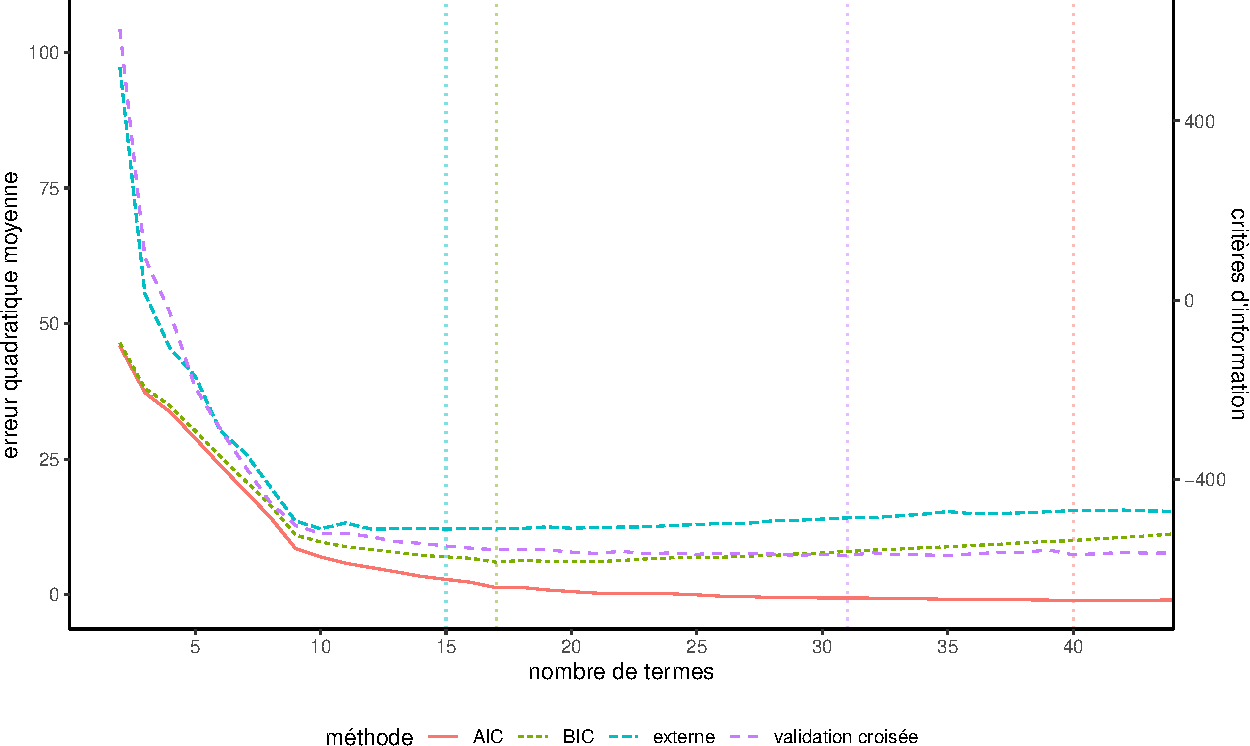
\includegraphics[width=0.8\textwidth,height=\textheight]{figures/fig-perfo-sequentiel.pdf}

}

\end{figure}

\footnotesize

40 premiers modèles de la procédure séquentielle en fonction du nombre
de termes inclus. Oracle: 100K données de validation (libellé externe)

\normalsize
\end{frame}

\begin{frame}{Méthodes de régularisation}
\protect\hypertarget{muxe9thodes-de-ruxe9gularisation}{}
Objectif: prévenir le surajustement.

L'erreur moyenne quadratique se décompose comme

\[ \text{biais carré} + \text{variabilité}\]

Les méthodes de régularisation introduisent du biais dans l'estimation
des coefficients en pénalisant leur norme.
\end{frame}

\begin{frame}{Préalable à la régression avec régularisation}
\protect\hypertarget{pruxe9alable-uxe0-la-ruxe9gression-avec-ruxe9gularisation}{}
Pénalisation la norme de \(\beta_1, \ldots, \beta_p\)

\begin{itemize}
\tightlist
\item
  Modèles avec pénalités pas les mêmes selon l'échelle des données

  \begin{itemize}
  \tightlist
  \item
    pas invariant aux transformations affines (par ex., conversion de
    Celcius en Farenheit)
  \end{itemize}
\end{itemize}

\textbf{Solution}: standardiser variables explicatives
\(\mathrm{X}_1, \ldots, \mathrm{X}_p\) \textbf{et} variable réponse
\(\boldsymbol{y}\) (moyenne zéro, écart-type unitaire).

\begin{itemize}
\tightlist
\item
  vérifier selon le logiciel, cette étape peut-être effectuée
  implicitement
\end{itemize}
\end{frame}

\begin{frame}{LASSO}
\protect\hypertarget{lasso}{}
Pénalité avec norme \(l_1\) pour la valeur absolue des coefficients,
\[ \min_{\boldsymbol{\beta}} \left\{ n\mathsf{EQM}(\boldsymbol{\beta}) + \lambda(|\beta_1| + \cdots + |\beta_p|)\right\}.\]
Hyperparamètre \(\lambda>0\) qui détermine la force de la pénalisation.

Rétrécissement de certains coefficients \textbf{exactement} à zéro:
sélection implicite de variable.
\end{frame}

\begin{frame}{Contrainte budgétaire et moindres carrés}
\protect\hypertarget{contrainte-budguxe9taire-et-moindres-carruxe9s}{}
\begin{figure}

{\centering 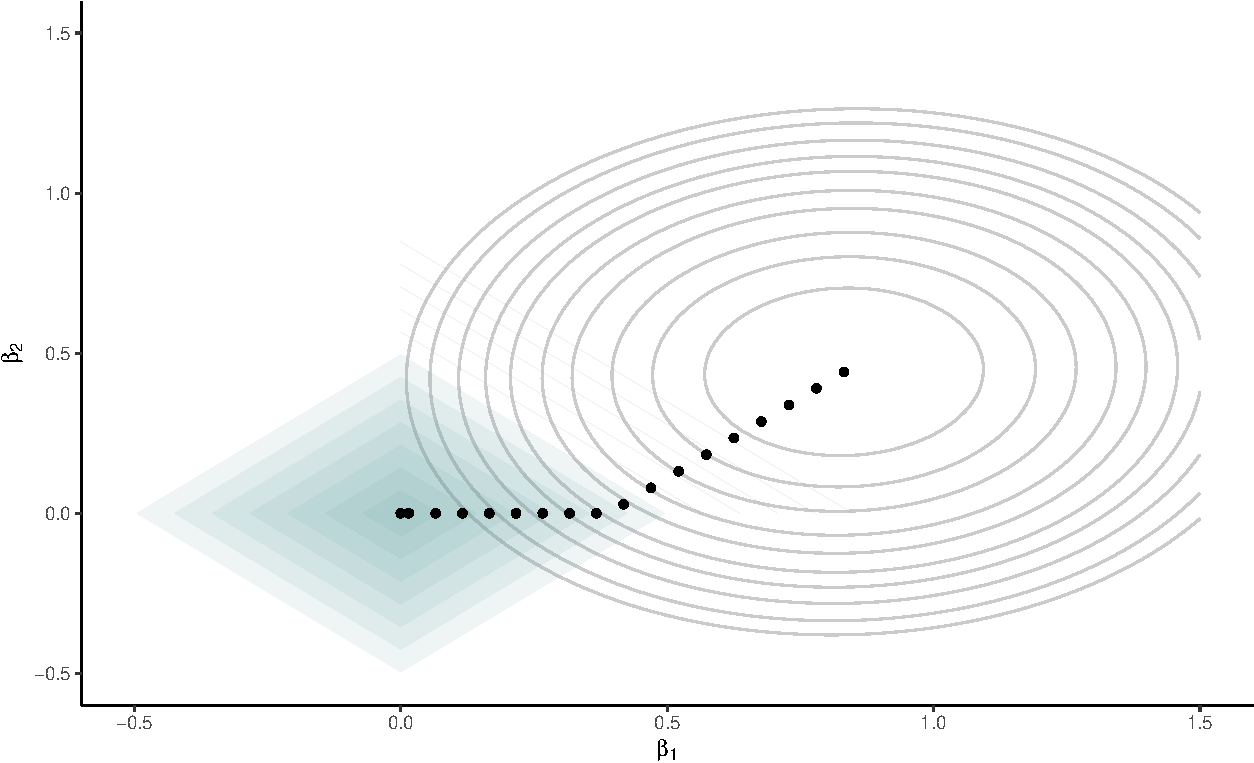
\includegraphics[width=0.8\textwidth,height=\textheight]{figures/fig-lassopenalty.pdf}

}

\end{figure}
\end{frame}

\begin{frame}[fragile]{Code \textbf{R} pour le LASSO}
\protect\hypertarget{code-r-pour-le-lasso}{}
Paramètre de pénalité déterminé par validation croisée à partir d'un
vecteur de valeurs candidates.

\begin{Shaded}
\begin{Highlighting}[numbers=left,,]
\FunctionTok{library}\NormalTok{(glmnet)}
\NormalTok{lambda\_seq }\OtherTok{\textless{}{-}} \FunctionTok{seq}\NormalTok{(}\AttributeTok{from =} \FloatTok{0.01}\NormalTok{, }\AttributeTok{to =} \DecValTok{2}\NormalTok{, }\AttributeTok{by =} \FloatTok{0.01}\NormalTok{)}
\NormalTok{cv\_output }\OtherTok{\textless{}{-}} 
\NormalTok{  glmnet}\SpecialCharTok{::}\FunctionTok{cv.glmnet}\NormalTok{(}\AttributeTok{x =} \FunctionTok{as.matrix}\NormalTok{(matmod), }
            \AttributeTok{y =}\NormalTok{ dbm\_a}\SpecialCharTok{$}\NormalTok{ymontant, }
            \AttributeTok{alpha =} \DecValTok{1}\NormalTok{, }
            \AttributeTok{lambda =}\NormalTok{ lambda\_seq)}
\FunctionTok{plot}\NormalTok{(cv\_output)}
\end{Highlighting}
\end{Shaded}
\end{frame}

\begin{frame}{Trajectoire LASSO}
\protect\hypertarget{trajectoire-lasso}{}
On choisit typiquement \(\lambda\) par validation croisée, soit

\begin{itemize}
\tightlist
\item
  le modèle avec la plus valeur de \(\mathsf{EQM}_{\mathrm{VC}}\).
\item
  le modèle le plus parsimonieux à au plus un erreur-type de ce dernier
  (pénalité plus élevée, plus de coefficients nuls)
\end{itemize}

\begin{figure}

{\centering 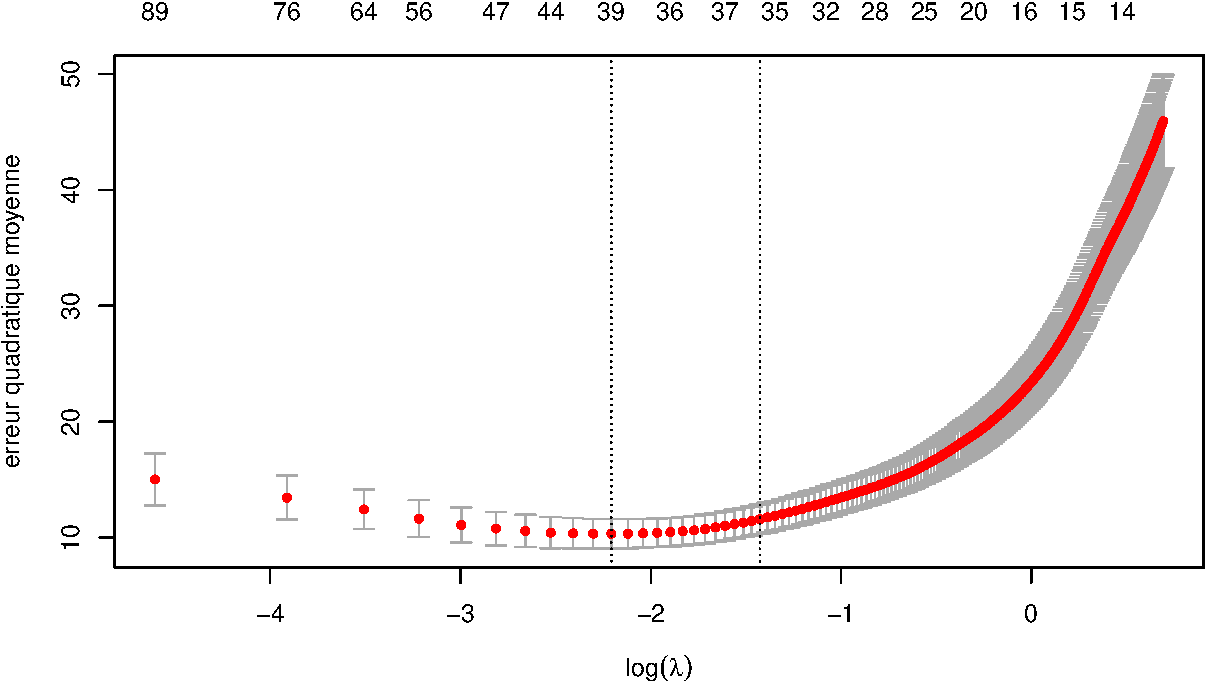
\includegraphics[width=0.8\textwidth,height=\textheight]{figures/fig-lassopath.pdf}

}

\end{figure}
\end{frame}

\begin{frame}{Paramètres}
\protect\hypertarget{paramuxe8tres}{}
\begin{figure}

{\centering \includegraphics[width=0.8\textwidth,height=\textheight]{MATH60602-diapos4_files/figure-beamer/fig-lassopath-1.pdf}

}

\caption{\label{fig-lassopath}Coefficients du modèle en fonction de la
pénalité}

\end{figure}
\end{frame}

\begin{frame}[fragile]{Évaluation et prédiction}
\protect\hypertarget{uxe9valuation-et-pruxe9diction}{}
Une fois la valeur de \(\lambda\) choisie, on réestime le modèle avec la
pénalité.

\begin{Shaded}
\begin{Highlighting}[numbers=left,,]
\NormalTok{lambopt }\OtherTok{\textless{}{-}}\NormalTok{ cv\_output}\SpecialCharTok{$}\NormalTok{lambda.min }
 \CommentTok{\#ou cv\_output$lambda.1se}
\NormalTok{lasso\_best }\OtherTok{\textless{}{-}} 
\NormalTok{  glmnet}\SpecialCharTok{::}\FunctionTok{glmnet}\NormalTok{(}
    \AttributeTok{x =} \FunctionTok{as.matrix}\NormalTok{(}\FunctionTok{as.matrix}\NormalTok{(matmod)),}
    \AttributeTok{y =}\NormalTok{ dbm\_a}\SpecialCharTok{$}\NormalTok{ymontant,}
    \AttributeTok{alpha =} \DecValTok{1}\NormalTok{, }
    \AttributeTok{lambda =}\NormalTok{ lambopt)}
\end{Highlighting}
\end{Shaded}
\end{frame}

\begin{frame}[fragile]{Prédictions}
\protect\hypertarget{pruxe9dictions}{}
On crée une matrice avec les données de validation et on calcule
l'erreur quadratique moyenne.

\footnotesize

\begin{Shaded}
\begin{Highlighting}[numbers=left,,]
\CommentTok{\# Prédictions et calcul de l\textquotesingle{}EQM}
\CommentTok{\# Données externes}
\NormalTok{dbm\_v }\OtherTok{\textless{}{-}}\NormalTok{ dbm }\SpecialCharTok{|\textgreater{}}
\NormalTok{  dplyr}\SpecialCharTok{::}\FunctionTok{filter}\NormalTok{(}
\NormalTok{    test }\SpecialCharTok{==} \DecValTok{1}\NormalTok{,}
    \SpecialCharTok{!}\FunctionTok{is.na}\NormalTok{(ymontant))}
\NormalTok{pred }\OtherTok{\textless{}{-}} \FunctionTok{predict}\NormalTok{(lasso\_best, }
                \AttributeTok{s =}\NormalTok{ lambopt, }
                \AttributeTok{newx =} \FunctionTok{as.matrix}\NormalTok{(}
                  \FunctionTok{model.matrix}\NormalTok{(formule, }
                               \AttributeTok{data =}\NormalTok{ dbm\_v)))}
\NormalTok{eqm\_lasso }\OtherTok{\textless{}{-}} \FunctionTok{mean}\NormalTok{((pred }\SpecialCharTok{{-}}\NormalTok{ dbm\_v}\SpecialCharTok{$}\NormalTok{ymontant)}\SpecialCharTok{\^{}}\DecValTok{2}\NormalTok{)}
\end{Highlighting}
\end{Shaded}

\normalsize
\end{frame}

\begin{frame}{Évaluation de la performance}
\protect\hypertarget{uxe9valuation-de-la-performance}{}
En incluant uniquement les variables de base

\begin{longtable}[]{@{}ccl@{}}
\toprule\noalign{}
nb variables & \(\mathsf{EQM}\) & méthode \\
\midrule\noalign{}
\endhead
15 & 25.69 & toutes les variables \\
12 & 25.53 & exhaustive - \(\mathsf{AIC}\) \\
10 & 25.04 & exhaustive - \(\mathsf{BIC}\) \\
\bottomrule\noalign{}
\end{longtable}

En incluant les termes de base, les carrés et les interactions d'ordre
2.

\begin{longtable}[]{@{}cll@{}}
\toprule\noalign{}
nb variables & \(\mathsf{EQM}\) & méthode \\
\midrule\noalign{}
\endhead
104 & 19.63 & toutes les variables \\
21 & 12 & séquentielle, choix selon \(\mathsf{AIC}\) \\
15 & 12.31 & séquentielle, choix selon \(\mathsf{BIC}\) \\
30 & 12 & LASSO, validation croisée avec 10 groupes \\
\bottomrule\noalign{}
\end{longtable}
\end{frame}

\begin{frame}{Récapitulatif}
\protect\hypertarget{ruxe9capitulatif}{}
\begin{itemize}
\tightlist
\item
  Le nombre de modèles possibles augmente rapidement avec le nombre de
  prédicteurs.
\item
  Si un modèle est mal spécifié (variables importantes manquantes),
  alors les estimations sont biaisées.
\item
  Si le modèle est surspécifié, les coefficients correspondants aux
  variables superflues incluses sont en moyenne nuls, mais contribuent à
  l'augmentation de la variance.
\item
  \textbf{Compromis biais/variance}.
\end{itemize}
\end{frame}

\begin{frame}{Récapitulatif}
\protect\hypertarget{ruxe9capitulatif-1}{}
\begin{itemize}
\tightlist
\item
  La taille du modèle (le nombre de variables explicatives) est
  restreinte par le nombre d'observations disponibles.
\item
  En général, il faut s'assurer d'avoir suffisamment d'observations pour
  estimer de manière fiable les coefficients
\item
  Porter une attention particulière aux variables binaires et aux
  interactions avec ces dernières: si les effectifs de certaines
  modalités sont faibles, il y a danger de surajustement.
\end{itemize}
\end{frame}

\begin{frame}{Récapitulatif}
\protect\hypertarget{ruxe9capitulatif-2}{}
\begin{itemize}
\tightlist
\item
  Une recherche exhaustive garantie le survol du plus grand nombre de
  modèles possibles, mais est coûteuse
\item
  On peut effectuer une recherche exhaustive à l'aide d'algorithmes
  d'optimisation pour un nombre réduit de variables (max 50)
\item
  Sinon, on a l'option d'utiliser un algorithme glouton qui ne couvre
  qu'un sous-ensemble de tous les modèles
\item
  Compromis coût de calcul vs nombre de modèles explorés
\item
  Possibilité de combiner des méthodes!
\end{itemize}
\end{frame}

\begin{frame}{Récapitulatif}
\protect\hypertarget{ruxe9capitulatif-3}{}
Certaines méthodes de pénalisation directe changent la fonction
objective:

\begin{itemize}
\tightlist
\item
  introduction de biais pour les coefficients.
\item
  idée globale: échanger biais contre variabilité moindre.
\end{itemize}

Une pénalité particulière (LASSO) contraint certains paramètres à être
exactement nuls,

\begin{itemize}
\tightlist
\item
  correspond implicitement à une sélection de variables.
\end{itemize}
\end{frame}

\begin{frame}{Récapitulatif}
\protect\hypertarget{ruxe9capitulatif-4}{}
\begin{itemize}
\tightlist
\item
  En pratique, on cherche à essayer le plus possible de bons modèles
  pour trouver le choix optimal de variables.
\item
  On applique le critère de sélection sur la liste de modèles candidats
  pour retenir celui qui donne la meilleure performance.
\end{itemize}
\end{frame}



\end{document}
